\section{迭代条件期望}
\label{sec:cexp-iterated}

条件期望$\mathbb{E}[X\mid\mathcal{G}]$本身是一个可积的随机变量，可以再对它求期望，或者再给定另一份信息求条件期望。这样平均两次，结果是什么？分两种情况：一种是第二次什么也不给定，条件被完全取消；另一种是第二次保留另一层信息。后一种情况能否化简，取决于两份信息之间有没有包含关系。

\subsection{全期望公式}
\label{sec:cexp-total-expectation}

\paragraph{先分组平均，再按组加权}
取消条件的情形最简单：在式~\eqref{eq:cexp-defining}中取$A=\Omega$。$\Omega$总在$\mathcal{G}$中，于是得到下面的定理。

\begin{theorem}[全期望公式]
\label{thm:cexp-total-expectation}
设$X$可积，$\mathcal{G}\subseteq\mathcal{F}$是$\sigma$代数。则
\begin{equation}
 \mathbb{E}\bigl[\mathbb{E}[X\mid\mathcal{G}]\bigr]=\mathbb{E}[X].
 \label{eq:cexp-total-expectation}
\end{equation}
\end{theorem}

\begin{proof}
在式~\eqref{eq:cexp-defining}中取$A=\Omega$，$\mathbf{1}_{\Omega}=1$。
\end{proof}

证明只有一行，含义却很具体。在有限划分中，$\mathbb{E}[X\mid\mathcal{G}]$在第$i$组取$c_i$，所以它的期望是$\sum_ic_i\mathbb{P}(A_i)$：先在每一组内求平均，再以各组的概率为权重把组平均加起来，就恢复了总平均。把概率看成质量，这就是“整体的重心等于各部分重心按质量加权的重心”。

传感器表上的计算见图~\ref{fig:cexp-total-expectation}。三行的质量依次是$0.3,0.4,0.3$，行内重心是$1/3,1,5/3$；把每行的质量集中到它的重心，再求这三个点的重心，
\[
 0.3\cdot\tfrac13+0.4\cdot1+0.3\cdot\tfrac53=0.1+0.4+0.5=1=\mathbb{E}[Y].
\]

\begin{BookInlineFigure}
  \centering
  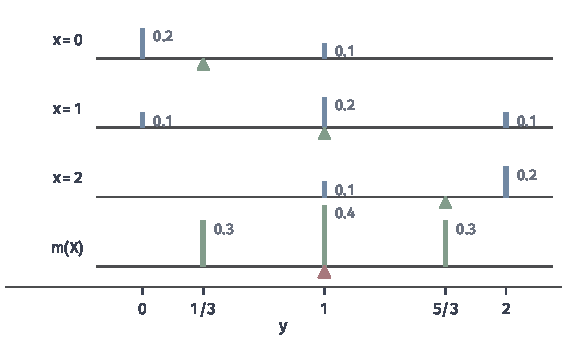
\includegraphics[width=96mm]{figures/07-probability/02-measure-theoretic-probability/matplotlib/cexp-total-expectation/figure.pdf}
  \caption{全期望公式是重心的合成，传感器表。上面三层是三行中的联合质量（蓝色竖线，高度与质量成正比），绿色三角是各行的重心$1/3$、$1$、$5/3$。最下一层把各行的质量$0.3$、$0.4$、$0.3$移到行重心（绿色竖线），它们的重心是$\mathbb{E}[Y]=1$（红色三角）。}
  \label{fig:cexp-total-expectation}
\end{BookInlineFigure}

逐次等分的例子同样可以核对。$\mathcal{G}_2$的四段各占$1/4$，段内平均是$\tfrac{1}{48},\tfrac{7}{48},\tfrac{19}{48},\tfrac{37}{48}$，于是
\[
 \mathbb{E}\bigl[\mathbb{E}[X\mid\mathcal{G}_2]\bigr]=\frac14\cdot\frac{1+7+19+37}{48}=\frac{64}{192}=\frac13=\int_0^1\omega^{2}\,\mathrm{d}\omega .
\]

\paragraph{统一求和与积分}
第~\ref{chap:random-vectors}章分别对概率表和联合密度证明了全期望公式，现在两者都是式~\eqref{eq:cexp-total-expectation}的特例。给定观测$Y$时，$\mathbb{E}[X\mid Y]=m(Y)$，由推前分布的积分公式，
\[
 \mathbb{E}[X]=\mathbb{E}\bigl[m(Y)\bigr]=\int m(y)\,P_Y(\mathrm{d}y).
\]
$Y$只取可数多个值时，右边是$\sum_ym(y)\,p_Y(y)$；$Y$有密度时，右边是$\int m(y)f_Y(y)\,\mathrm{d}y$。两种计算方式只是对$P_Y$积分的两种具体写法。

全期望公式在没有密度时同样好用。“只知绝对值”的例子中，由式~\eqref{eq:cexp-folding}，$\mathrm{e}^{X}$给定$\lvert X\rvert$的条件期望是$\cosh\lvert X\rvert$，而$\lvert X\rvert\sim\operatorname{Unif}(0,1)$，于是
\[
 \mathbb{E}[\mathrm{e}^{X}]=\mathbb{E}\bigl[\cosh\lvert X\rvert\bigr]=\int_0^1\cosh y\,\mathrm{d}y=\sinh 1 .
\]
直接计算得到同样的结果：
\[
 \mathbb{E}[\mathrm{e}^{X}]=\frac12\int_{-1}^{1}\mathrm{e}^{x}\,\mathrm{d}x=\frac{\mathrm{e}-\mathrm{e}^{-1}}{2}=\sinh1 .
\]
先把对称的两点合并，被积函数变成偶函数$\cosh$，积分区间减半；这正是先分组平均、再对组求平均的计算方式。

\subsection{塔式法则}
\label{sec:cexp-tower}

\paragraph{嵌套的信息}
现在第二次平均也保留一些信息。设$\mathcal{H}\subseteq\mathcal{G}$：$\mathcal{H}$中的事件都能由$\mathcal{G}$判断，$\mathcal{H}$是较少的信息。有限划分时，这表示$\mathcal{H}$的每一组都是$\mathcal{G}$的若干组之并，即$\mathcal{G}$是$\mathcal{H}$的细分。

传感器表中取$\mathcal{G}=\sigma(X)$，再取$\mathcal{H}=\sigma(\mathbf{1}_{\{X=2\}})$，后者只知道第一台“是否读偏高”，把前两行并成一组$\{X\leq1\}$，第三行单独一组。先按行平均，再在$\mathcal{H}$的组内平均：$\{X\leq1\}$的概率是$0.7$，其中前两行的质量分别是$0.3$与$0.4$，于是
\[
 \mathbb{E}\bigl[\mathbb{E}[Y\mid X]\bigm|\mathcal{H}\bigr]=\frac{0.3\cdot\frac13+0.4\cdot1}{0.7}=\frac{0.5}{0.7}=\frac57\quad\text{在}\ \{X\leq1\}\ \text{上}.
\]
另一方面，直接在$\{X\leq1\}$上求$Y$的平均，五个正概率格子上的累计期望是$0.1+0.4=0.5$，同样得$5/7$。第三行在两种算法下都是$5/3$。图~\ref{fig:cexp-tower-nested}画出了这两条路径。

\begin{BookInlineFigure}
  \centering
  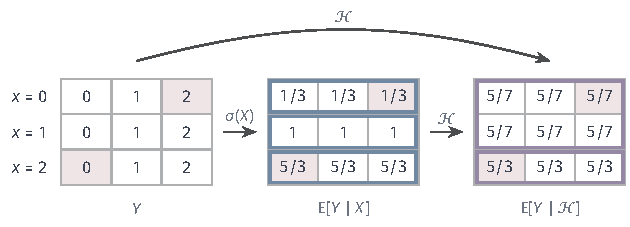
\includegraphics[width=106mm]{figures/07-probability/02-measure-theoretic-probability/tikz/cexp-tower-nested/figure.pdf}
  \caption{嵌套信息下的塔式法则，传感器表，浅红格概率为零。左：$Y$在九个格子上的值。中：$\mathbb{E}[Y\mid X]$，在每行（蓝框）取常数。右：$\mathbb{E}[Y\mid\mathcal{H}]$，$\mathcal{H}=\sigma(\mathbf{1}_{\{X=2\}})$的两组（紫框）上分别取$5/7$与$5/3$。下方两步与上方一步得到相同的结果。}
  \label{fig:cexp-tower-nested}
\end{BookInlineFigure}

\paragraph{先细后粗与先粗后细}
两种顺序都得到较粗信息上的条件期望。

\begin{theorem}[塔式法则]
\label{thm:cexp-tower}
设$X$可积，$\mathcal{H}\subseteq\mathcal{G}\subseteq\mathcal{F}$都是$\sigma$代数。则
\begin{equation}
 \mathbb{E}\bigl[\mathbb{E}[X\mid\mathcal{G}]\bigm|\mathcal{H}\bigr]=\mathbb{E}[X\mid\mathcal{H}]
 =\mathbb{E}\bigl[\mathbb{E}[X\mid\mathcal{H}]\bigm|\mathcal{G}\bigr].
 \label{eq:cexp-tower}
\end{equation}
\end{theorem}

\begin{proof}
\emph{先细后粗。}记$Z=\mathbb{E}[X\mid\mathcal{G}]$，它可积。要证$\mathbb{E}[X\mid\mathcal{H}]$是$\mathbb{E}[Z\mid\mathcal{H}]$的一个版本。它是$\mathcal{H}$可测且可积的；对$A\in\mathcal{H}$，因为$\mathcal{H}\subseteq\mathcal{G}$，$A$也在$\mathcal{G}$中，两次使用式~\eqref{eq:cexp-defining}，
\[
 \mathbb{E}[Z\mathbf{1}_{A}]=\mathbb{E}[X\mathbf{1}_{A}]=\mathbb{E}\bigl[\mathbb{E}[X\mid\mathcal{H}]\,\mathbf{1}_{A}\bigr].
\]
第一个等号用了$A\in\mathcal{G}$，第二个等号用了$A\in\mathcal{H}$。

\emph{先粗后细。}$\mathbb{E}[X\mid\mathcal{H}]$是$\mathcal{H}$可测的，因而也是$\mathcal{G}$可测的，并且可积。由定理~\ref{thm:cexp-known}的最后一句，给定$\mathcal{G}$对它求条件期望，结果是它自身。
\end{proof}

式~\eqref{eq:cexp-tower}称为\term{塔式法则}（tower property）。两个等号的来源不同。先细后粗用的是积分定义：较粗信息下的已知事件，在较细信息下也是已知的，累计期望在两层平均中都被保留。先粗后细用的是“已知量不变”：粗信息下的平均在细信息下已经是已知量，再平均也不改变。两者合起来，迭代的结果总是较粗的那一层，较少的信息胜出。全期望公式是$\mathcal{H}=\{\emptyset,\Omega\}$的特例。

\paragraph{没有包含关系时}
塔式法则依赖$\mathcal{H}\subseteq\mathcal{G}$。两份信息互不包含时，迭代的顺序会影响结果，也不能换成在两者共有的信息上求平均。仍用传感器表，取$\sigma(X)$（按行分组）与$\sigma(D)$（按对角线分组，$D=X-Y$）。

先按行平均，再按对角线平均。$\mathbb{E}[Y\mid X]$在$D=1$的两格$(1,0)$与$(2,1)$上分别取$1$与$5/3$，两格概率相等，于是在$\{D=1\}$上
\[
 \mathbb{E}\bigl[\mathbb{E}[Y\mid X]\bigm|D\bigr]=\frac12\Bigl(1+\frac53\Bigr)=\frac43 .
\]
同样算得$\{D=0\}$上为$1$，$\{D=-1\}$上为$2/3$，见图~\ref{fig:cexp-tower-non-nested}(a)。

反过来，先按对角线平均，再按行平均。$\mathbb{E}[Y\mid D]$在第一行的两个正概率格子$(0,0)$与$(0,1)$上分别取$1$与$3/2$，两格概率为$0.2$与$0.1$，于是在$\{X=0\}$上
\[
 \mathbb{E}\bigl[\mathbb{E}[Y\mid D]\bigm|X\bigr]=\frac{0.2\cdot1+0.1\cdot\frac32}{0.3}=\frac76 .
\]
另外两行分别得到$1$与$5/6$，见图~\ref{fig:cexp-tower-non-nested}(b)。

\begin{BookInlineFigure}
  \centering
  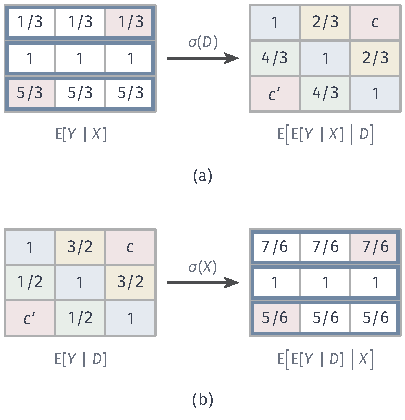
\includegraphics[width=68mm]{figures/07-probability/02-measure-theoretic-probability/tikz/cexp-tower-non-nested/figure.pdf}
  \caption{互不包含的两份信息，传感器表。蓝框表示按行（$\sigma(X)$）取常数，同色格子表示按对角线（$\sigma(D)$，$D=X-Y$）取常数，$c$、$c'$是零概率组上的任意常数。(a)先给定$X$再给定$D$。(b)先给定$D$再给定$X$。两个结果不同，也都不是常数$\mathbb{E}[Y]=1$。}
  \label{fig:cexp-tower-non-nested}
\end{BookInlineFigure}

两种顺序的结果一个是$D$的函数，一个是$X$的函数，彼此不同。它们也都不等于在共同信息$\sigma(X)\cap\sigma(D)$上的平均：一个事件若同时是若干整行之并和若干整条对角线之并，只要含有某一行，就含有这一行经过的对角线，进而含有那些对角线经过的其他行，最后只能是$\Omega$；所以共同信息只有$\{\emptyset,\Omega\}$，相应的平均是常数$1$。两份信息各自有用，交起来却什么也不剩，先后两次平均在两种顺序下也都没有抵达这个常数。
